% \section{Sistemas Binarios}
\chapter{Sistemas Binarios}

La gran mayoría de sistemas estelares dentro de nuestra Galaxia no son aquellos
solitarios como nuestro propio sistema solar, si no que son compuestas de dos o
más estrellas ubicadas en corta aproximación de una a otra, a ordenes de
unidades astronómicas (AU por sus siglas en inglés). Estos sistemas multiples se
pueden clasificar con mayor precisión para aquellos compuestos de solo dos
estrellas, denominados como \textit{sistemas binarios}. Dentro de un sistema
binario la corta separación orbital entre ambas estrellas da como consecuencia a
fenómenos que surgen mediante la interacción entre las componentes, tanto como
la interacción gravitacional debido a sus masas, como a la física interesante
que ocurre en el caso de interacciones de material entre una estrella a otra. 

% TODO: incluir sección en cite?
Los sistemas binarios estelares ofrecen un laboratorio celeste de gran
importancia, ya que debido a la interacción a cortas escalas espaciales nos
brindan información acerca de las estrellas que sería imposible obtener de otra
manera. \citetbookchapter{phoebeScientificReference}{2.1} menciona varios
parámetros derivados de observaciones de estos sistemas, como las masas de cada
una de las componentes estelares por medio de su interacción gravitacional, la
calibración y estudio de la evolución estelar y su dependencia de la masa y
luminosidad de la estrella; dadas observaciones de sistemas desconectados, en el
cual ambas componentes son de la misma edad pero con diferentes propiedades que
influyen su camino evolutivo. La clasificación de estos sistemas se basa tanto
en propiedades observacionales\textemdash las cuales dependen tanto de las
propiedades geométricas del sistema como de nuestra capacidad de observación, en
cuanto a la capacidad de la instrumentación disponible\textemdash como en las
propiedades físicas del sistema, incluyendo la proximidad de las componentes
como sus propiedades lumínica.

\section{Geometría del Sistema - Modelo de Roche}

Es importante entender la forma geométrica de un sistema binario para llegar a
una descripción adecuada de ellos. Esto incluye los parámetros orbitales de las
estrellas tanto como la forma misma de ambas componentes, ya que en ciertos
casos tratar las estrellas como esferas rígidas da como resultado un modelo
incorrecto. A continuación se introduce las bases de las cuales se parte para
llegar a una representación de un sistema modelo, llegando a describir el
\textbf{modelo de Roche}.

Se define un sistema de coordenadas cartesiano tridimensional considerando un
marco de referencia no inercial, el cual está rotando con la misma velocidad que
las componentes del sistema binario orbitan una a otra. Esta es una
representación típica para el \textit{problema de tres cuerpos}, en el cual
tenemos a dos objetos masivos cuya influencia gravitacional se extiende al
espacio representado por el sistema de coordenadas. En la
\reffigure{figuraTresCuerpos} se puede ver este esquema, donde $m_1$ y $m_2$
representan ambas componentes estelares, posicionadas de tal manera que la
distancia entre las estrellas solo tenga una componente en una dirección
cartesiana.

\begin{figure}
	\centering
	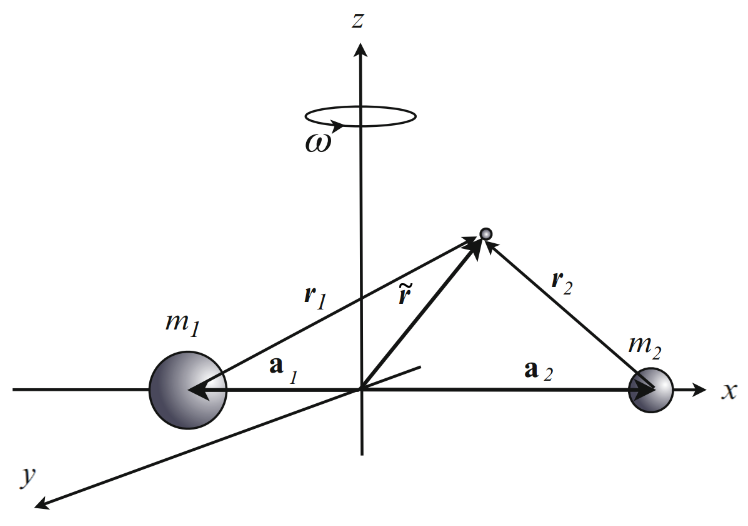
\includegraphics[scale=0.4]{Introduccion/Figures/Figura Tres Cuerpos_Intro Evolution Single Binary Stars.png}
	\caption{Configuración del problema de tres cuerpos dados dos objetos de
	alta masa $m_1$ y $m_2$ (las cuales representan cada componente estelar del
	sistema binario), y una partícula de masa despreciable de prueba ubicada a
	una distancia $r_1$ y $r_2$ de las estrellas respectivamente. El centro de
	masa del sistema está ubicado en el origen del sistema de coordenadas;
	\citetbookchapter{phoebeScientificReference}{3.1} posiciona la componente
	$m_1$ en el origen, con tal de simplificar las expresiones del modelo.
	Figura obtenida de
	\citetbookchapter{benacquista_introduction_to_evolution_single_binary_stars_2013}{13.1}.}
	\label{figuraTresCuerpos}
\end{figure}

La \reffigure{figuraTresCuerpos} define el sistema de coordenadas rotando junto
al sistema binario. La velocidad angular de Kepler está dada por:

\begin{eqfloat}
	\centering
	\begin{equation}
		\omega = \frac{2 \pi}{P_{orb}} = \sqrt{\frac{G (m_1 + m_2)}{a^3}}
	\end{equation}
	\blankcaption
	\label{ecuacionVelocidadAngular}
\end{eqfloat}

Donde $G = 6.673 \times 10^{-11} \ \mathrm{m}^3 \mathrm{kg}^{-1}
\mathrm{s}^{-2}$ es la constante de gravitación universal, $P_{orb}$ es el
periodo orbital de las estrellas (el cual es igual para ambas estrellas de
acuerdo con la segunda ley de Kepler), y $a = a_1 + a_2$ es el semieje mayor.
Usando la \refequation{ecuacionVelocidadAngular} podemos definir el Lagrangiano
para una partícula de prueba con masa $m$, el cual está a una distancia
$\mathbf{r}_1$ y $\mathbf{r}_2$ de $m_1$ y $m_2$ respectivamente, y a una
distancia $\mathbf{r}$ del centro de masa del sistema:

\begin{eqfloat}
	\centering
	\begin{equation}
		\Lagr = \eqnmark[MyDarkRed]{node1}{\frac{1}{2} m (\dot{x}^2 + \dot{y}^2) + \dot{z}^2}  +
				\eqnmark[MyDarkGreen]{node2}{\frac{1}{2} m \omega^2 (x^2 + y^2)} +
				\eqnmark[MyDarkBlue]{node3}{\frac{G m_1 m}{r_1} + \frac{G m_2 m}{r_2}}		
	\end{equation}
	\blankcaption
	\label{ecuacionLagrangianoTresCuerpos}
\end{eqfloat}

\section{Clasificaciones Observacionales}

Dependiendo del método de detección y las propiedades aparentes del sistema se
puede clasificar un sistema binario de estrellas. Estas clasificaciones son
independiente de sus propiedades físicas, como la clase espectral de cada
estrella o sus masas individuales. Al determinar su clasificación observacional
se puede delimitar las técnicas observacionales que son viables para recabar
datos del sistema; un sistema astrométrico sería indistinguible de uno
espectroscópico si uno intenta identificar las componentes individuales a simple
vista, o con un telescopio demasiado débil para el trabajo.

Las \textbf{binarias visuales} son aquellos cuya separación orbital aparente es
suficientemente grande para distinguir las dos estrellas individuales en la
bóveda celeste. A pesar de que se puede trazar la órbita de la secundaria con
varios años de observaciones, se requiere de cálculos adicionales para
determinar la órbita exacta de las componentes. Esto se debe a la inclinación
del sistema con respecto al eje de observación hacia la Tierra; solo es posible
observar \quotes{una proyección del elipse orbital relativo en el plano del
cielo,} aunque esto se puede superar usando el hecho de que la estrella primaria
aparentemente inmóvil debe de estar presente \quotes{en un punto focal de la
órbita relativa.} \citetbookchapter{fundamentalAstronomy}{10}

Las \textbf{binarias espectroscópicas} presentan variaciones periódicas en sus
espectros, en donde las líneas espectrales detectadas \quotes{oscilan
periodicamente alrededor de la longitud de onda promedio}
\citetbookchapter{astronomyPhysicalPerspective}{5}. Esto se observa
debido al \textit{desplazamiento de Doppler}, lo cual causa que la frecuencia de
un fotón se recorra hacia frecuencias más pequeñas (azules) o más grandes
(rojas) dependiendo de su velocidad radial con respecto al observador, si se va
acercando o alejando, respectivamente. Estas también pueden identificadas al
observar dos distintos grupos de líneas espectrales, el cual es resultado de la
contribución de ambas estrellas.

Las \textbf{binarias astrométricas}, al igual que las espectroscópicas, solo
muestran una componente visible al ser observada, al contrario de las binarias
visibles. Sin embargo, una binaria astrométrica difiera de las otras dos
categorías definidas en cuestión de su movimiento observado en la bóveda
celeste. Estas muestran un movimiento errático y no-lineal, algo que no se
esperaría ver en una estrella solitaria dado su inercia según la primera ley de
Newton. Estas perturbaciones son causadas por una estrella secundaria no
aparente al observar el sistema. 

\section{Binarias Eclipsantes}

Una de las propiedades más importantes de identificar de un sistema binario es
la \textit{inclinación} de su órbita con respecto a nuestra línea de visión
desde el sitio de observación (ya sea la Tierra en caso de un observatorio
terrestre o un punto lejano dentro del sistema solar para un telescopio
espacial). En dado caso que un sistema tenga una inclinación suficientemente
alta se pueden observar eclipses dentro del sistema, en lo que una componente
obscurece a su compañera de nuestra línea de visión. Estos eclipses se
manifiestan como disminuciones en el flujo total del sistema, brindando
información que no se obtendría sin esta perspectiva visual. 

\section{Binarias en Contacto}